\chapter{复合物筛选模型设计}
\label{chapter:gcnfilter}

\section{相关算法介绍}
\label{section:arithmetic}
\subsection{网络嵌入}
\label{subsection:nodeEmbedding}
\subsection{图卷积神经网络}
\label{subsection:GCN}
\subsection{图自编码器}
\label{subsection:GAE}
\section{算法总体流程}
\label{section:progress}

复合物筛选模型框架设计如图\ref{fig:main-process}所示;

\begin{figure}[htbp]
    \centering
    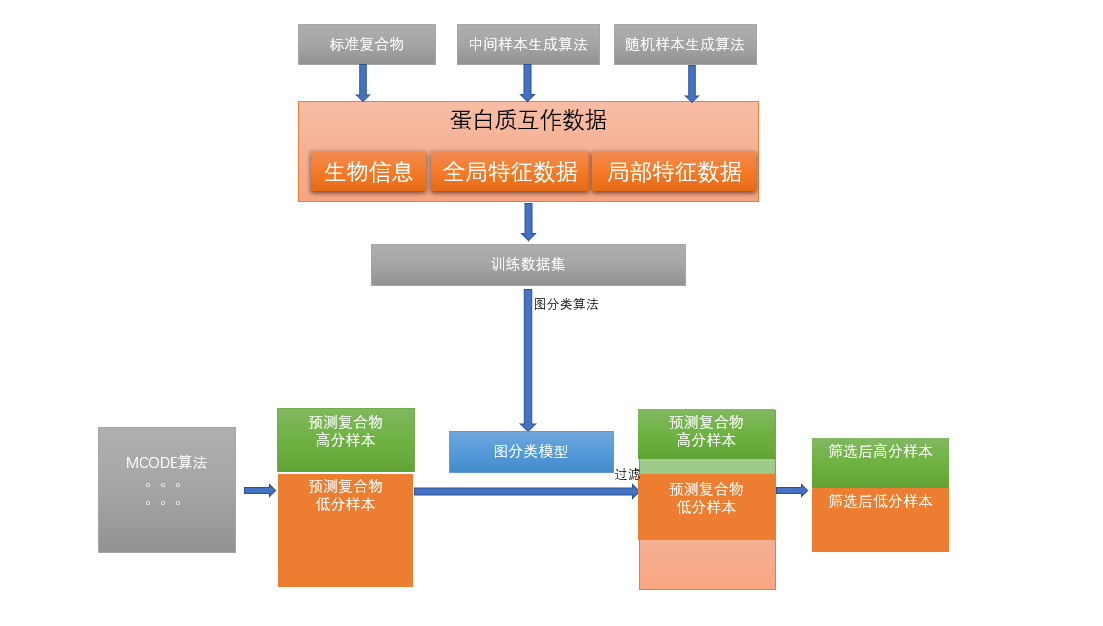
\includegraphics[width=14cm]{main-process}
    \caption{复合物筛选框架主体流程图}
    \label{fig:main-process}
\end{figure}

首先依照\label{section:datasetExtract}提出的数据集构建方法,对每一个复合物网络可以得到一个由复合物子图构成的数据集。该数据集中每一个复合物子图有和标准复合物的邻居相似性评分,总体分为四类复合物,分别为标准复合物、高评分预测复合物、低评分预测复合物和随机复合物。

第一阶段,提出合适的复合物筛选模型,并基于该数据集训练复合物分类模型\ref{section:GlobalfeatBaseModel}。

第二阶段,在蛋白质相互作用网络中得到复合物预测算法,如MCODE算法、clique算法等的预测结果。依据复合物分类结果的评价方法,在这些预测结果中,有一部分高分样本复合物预测符合预期结果,如图中绿色部分所示,其余部分为低分复合物样本,如图中红色部分所示。下一步利用复合物分类模型对所有的样本进行筛选,通过筛选的复合物符合模型学习到的复合物一般分布规律,筛选之后保留的复合物如图最终输出结果所示。

第三阶段,本文使用多种的复合物预测评价指标对筛选前后的总体样本进行综合评价。


\section{基于全局特征的模型}
\label{section:GlobalfeatBaseModel}




\section{基于生物特征的模型}
\label{section:biofeatBaseModel}

生物上的,拓扑上的,异常数据处理,过大数据归一化

GAE怎么做的,deepwalk怎么做的,node2vec怎么做的
\section{特征融合模型}
\label{section:fusionfeatBaseModel}
考虑少量蛋白质特征,考虑图拓扑特征,图拓扑特征的计算参考\cite{yu_predicting_2014}
\section{尺寸敏感性的图读出算法}
\label{section:GPool}
